\documentclass[12pt]{article}

\usepackage{a4wide}
\usepackage[utf8]{inputenc}
\usepackage{hyperref}
\usepackage{graphicx}
\usepackage{amsmath}

%\parindent=0pt
\begin{document}

\section*{SLIC Algorithm for Image Segmentation}

This exercise is focused on implementation of SLIC (Simple Linear Iterative Clustering) algorithm.
This algorithm is inspired by the $k$-means algorithm, and its goal is to cluster image pixels into segments (clusters) based on their color similarity and proximity in the image plane (see Figure~\ref{img1}).

Similarly as in the $k$-means, SLIC takes as input a desired number of segments $K$.
For an image with $N$ pixels, the approximate size of each segment is therefore $N/K$ pixels. 
For roughly equally sized segments there would be a segment center $C$ at every grid interval $S = \sqrt{N/K}$.
The segment center $C_k$ is represented as 5D vector $[R_k, G_k, B_k, x_k, y_k]$ for $k=1, 2, \ldots, K$ (in the original paper \cite{slic}, the authors use CIELAB color space, you can use it as well).

\begin{figure}[h]
\centering
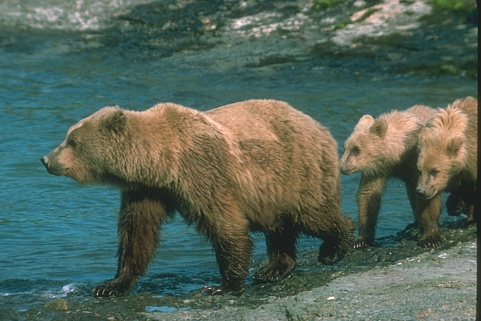
\includegraphics[width=0.45\textwidth]{images/100075}
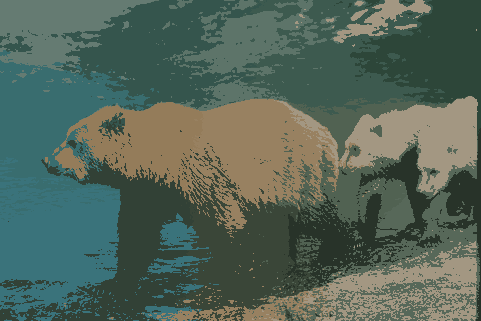
\includegraphics[width=0.45\textwidth]{images/img_res}
\caption{The input image (\textit{left}) and its segmentation (\textit{right}).}
\label{img1}
\end{figure}

In the first step, $K$ segment centers are regularly sampled on the image plane and moved to the locations corresponding to the lowest gradient position in a $3 \times 3$ neighborhood (Figure~\ref{img2}(\textit{left})).
This is done to avoid placing the center at an edge and to reduce the chances of choosing a noisy pixel (you can use the edge detection algorithm from the previous lectures). 
Afterwards, each image pixel is assigned to one of the segment based on the distance, i.e. the distance from a pixel $i$ to all the segment centers is computed, and the pixel is assigned to the segment whose center has the lowest distance to $i$.
The algorithm assumes that pixels that are associated with a segment lie within a $2S \times 2S$ area around the center of this segment on the $xy$ plane.
This step reduces the search space.
The distance measure $D_S$ is defined as the sum of the distance in color space $d_{RGB}$ and the distance in spatial space $d_{xy}$ normalized by the grid interval $S$:
\begin{align}
d_{RGB} &= \sqrt{(R_k-R_i)^2+(G_k-G_i)^2+(B_k-B_i)^2} \\
d_{xy} &= \sqrt{(x_k-x_i)+(y_k-y_i)^2} \\
\label{eq1}
D_s &= d_{RGB} + \frac{m}{S} d_{xy}.
\end{align}
A variable $m$ is used to set the balance between the color and spatial distances (you can experiment with this value).

After all the pixels are associated with the nearest cluster center, a new center is computed as the average $[R, G, B, x, y]$ vector of all the pixels belonging to the cluster. 
This process of associating pixels with the nearest cluster center and recomputing the center is iteratively repeated until convergence.

\subsubsection*{Algorithm}

\begin{enumerate}
    \item Initialize cluster centers $C_k = [R_k, G_k, B_k, x_k, y_k]$ by sampling pixels at regular grid steps $S$ and move the cluster centers to the lowest gradient position in a $3\times 3$ neighborhood.
    \item For each cluster center $C_k$, assign the pixels from a $2S \times 2S$ square neighborhood around the cluster center $C_k$ according to the distance $D_S$ (Equation~\ref{eq1}).
    \item Compute new cluster centers as the average vectors of all the pixels belonging to the cluster.
    \item Repeat from step 2 until the cluster centers do not move very much (distance is less that a given threshold).
\end{enumerate}

\begin{figure}
\centering
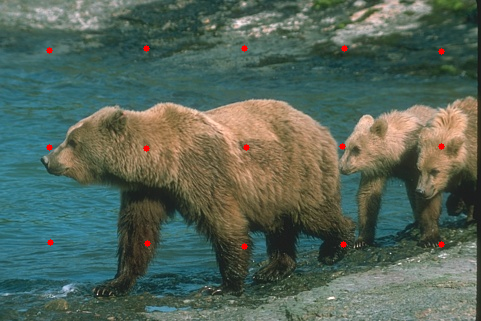
\includegraphics[width=0.45\textwidth]{images/img1}
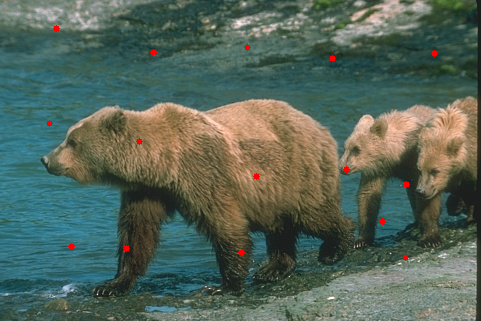
\includegraphics[width=0.45\textwidth]{images/img2}
\caption{The segment centers (red dots) in the first iteration (\textit{left}) and after convergence (\textit{right}).}
\label{img2}
\end{figure}

\begin{thebibliography}{99}
\bibitem{slic}
Radhakrishna Achanta, Appu Shaji, Kevin Smith, Aurelien Lucchi, Pascal Fua, and Sabine S{\"u}sstrunk, \emph{SLIC Superpixels}, EPFL Technical Report 149300, June 2010.
\bibitem{video}
\emph{How SLIC (Simple Linear Iterative Clustering) algorithm works}. 2018.\\
\url{https://www.youtube.com/watch?v=-hmUbB-Y8R0}
\end{thebibliography}

\end{document}

